%% chapter10_multi_agent_setting_slides.tex
%% Beamer slides for Chapter 10: Multi-Agent Setting
%% An Introduction to Universal Artificial Intelligence (2024)
%% Hutter, Quarel, Catt -- Taylor & Francis / CRC Press
%% Reader-friendly style: complete sentences, symbol explanations, worked examples
%% Compiled with: pdflatex -interaction=nonstopmode chapter10_multi_agent_setting_slides.tex  (twice)
\documentclass[aspectratio=169,10pt]{beamer}

\usetheme{Madrid}
\usecolortheme{seahorse}

%% ── Packages ──────────────────────────────────────────────────────────────
\usepackage{amsmath,amssymb,amsfonts}
\usepackage{mathtools}
\usepackage{graphicx}
\usepackage{booktabs}
\usepackage{xcolor}
\usepackage{listings}
\usepackage{tikz}
\usetikzlibrary{arrows.meta,positioning,shapes.geometric,fit,backgrounds}

\graphicspath{{figures/}}

%% ── Python listing style ─────────────────────────────────────────────────
\lstdefinestyle{pycode}{
  language=Python,
  basicstyle=\ttfamily\scriptsize,
  numbers=left,
  numberstyle=\tiny\color{gray},
  frame=single,
  backgroundcolor=\color{gray!7},
  keywordstyle=\color{blue!70!black}\bfseries,
  commentstyle=\color{green!50!black}\itshape,
  stringstyle=\color{orange!80!black},
  showstringspaces=false,
  breaklines=true,
  tabsize=4,
  xleftmargin=1.5em,
  framexleftmargin=1.5em,
  aboveskip=4pt,
  belowskip=4pt,
}

%% ── Metadata ─────────────────────────────────────────────────────────────
\title[Ch.\,10 Multi-Agent Setting]{%
  \textbf{Chapter 10: Multi-Agent Setting}\\
  \normalsize An Introduction to Universal Artificial Intelligence}
\subtitle{Utilities, Game Theory, Reflective Oracles, and the Grain of Truth}
\author{Marcus Hutter, Elliot Catt, David Quarel}
\institute{Taylor \& Francis / CRC Press, 2024}
\date{}

\setbeamertemplate{footline}[frame number]
\setbeamertemplate{navigation symbols}{}

%% Helpful macros
\newcommand{\R}{\mathbb{R}}
\newcommand{\N}{\mathbb{N}}
\newcommand{\B}{\mathbb{B}}
\newcommand{\Pb}{\mathbb{P}}
\newcommand{\E}{\mathbb{E}}
\newcommand{\Mc}{\mathcal{M}}
\newcommand{\Ac}{\mathcal{A}}
\newcommand{\Ec}{\mathcal{E}}
\newcommand{\Oc}{\mathcal{O}}
\newcommand{\Nc}{\mathcal{N}}
\newcommand{\Tc}{\mathcal{T}}
\newcommand{\hlt}{h_{<t}}

%% ══════════════════════════════════════════════════════════════════════════
\begin{document}

%% ── Title frame ──────────────────────────────────────────────────────────
\begin{frame}
  \titlepage
\end{frame}

%% ── Outline ──────────────────────────────────────────────────────────────
\begin{frame}{Chapter Overview}
  \tableofcontents
\end{frame}

\AtBeginSection[]{\begin{frame}{Outline}\tableofcontents[currentsection]\end{frame}}

%% ══════════════════════════════════════════════════════════════════════════
\section{10.1 From Preferences to Utilities}

\begin{frame}{Why a Multi-Agent Chapter?}
  So far this book has only discussed the \textbf{single-agent} setting,
  where there is one agent and the environment. More realistically, and
  more complex, is the \textbf{multi-agent setting}, where we consider the
  agent, the environment, \emph{and} some number of other agents.

  \vspace{0.4em}
  \textbf{Why not just fold the other agents into the environment?} We
  could try to capture the behaviour of other agents as part of the
  environment. While this is technically possible, it misses some of the
  subtlety and advantages of explicitly considering the multi-agent
  setting: when we \emph{know} we are facing other agents, we know they will
  also learn, or at least act in specific, structured ways with respect to
  our own actions -- and we can try to exploit that structure.

  \vspace{0.4em}
  \textbf{Roadmap for this chapter.}
  \begin{itemize}
    \item \textbf{10.1} A classic decision-theory result: rational
      preferences can be represented by a real-valued (von
      Neumann--Morgenstern) \emph{utility function} -- the basis of
      expected utility theory and hence most of game theory.
    \item \textbf{10.2} The basics of \textbf{game theory}: strategic
      games, Nash equilibrium, and five famous $2\times2$ games.
    \item \textbf{10.3--10.4} How multi-agent \emph{extensive-form} games
      relate to (history-based) reinforcement learning.
    \item \textbf{10.5--10.7} \textbf{Reflective oracles}, the
      \textbf{grain of truth} problem, and \textbf{Reflective AIXI} --
      how to let agents reason about opponents that may themselves be
      reasoning about them, without an infinite regress.
  \end{itemize}
\end{frame}

\begin{frame}{Preferences and Lotteries}
  We would like to formalize what it means for an agent to be
  \textbf{rational}. Let $\Oc$ (calligraphic $O$) denote a set of
  \textbf{outcomes} (this could even be the set of all finite interaction
  histories), and let $\prec$ (``precedes'', pronounced ``is preferred
  less than'') denote the agent's \textbf{preference}, a binary relation
  over $\Oc$.

  \vspace{0.4em}
  In practice, a full description of the preferences $\prec$ of an agent
  (like a human) may in general be unknown. We treat the agent's
  preferences as a black box, and assume we can \emph{query} the agent: if
  the agent strictly prefers $a$ to $b$ we write $a\succ b$, or $b\prec a$.
  If the agent is indifferent between $a$ and $b$ (formally, $a\not\succ b$
  and $b\not\succ a$) we write $a\sim b$. The symbols $\succeq$ and
  $\preceq$ (``at least as preferred as'' / ``no more preferred than'')
  are defined in the obvious fashion.

  \vspace{0.4em}
  \textbf{Lotteries.} Given two outcomes $a,b\in\Oc$ and $\theta$ (Greek
  letter \emph{theta}) $\in[0,1]$, we define a \textbf{lottery}
  $\theta a+(1-\theta)b$ as the random outcome representing: observe
  outcome $a$ with probability $\theta$, and outcome $b$ with probability
  $1-\theta$. We require that $\Oc$ is \emph{closed under lotteries}, and
  that the agent also has preferences defined for lotteries -- that is,
  given any outcomes $a,a',b,b'\in\Oc$ and $\alpha,\beta\in[0,1]$
  ($\alpha$ = ``alpha'', $\beta$ = ``beta''), the outcomes
  $\alpha a+(1-\alpha)a'$ and $\beta b+(1-\beta)b'$ are themselves in
  $\Oc$, and hence comparable with respect to $\prec$. This is what makes
  outcomes \emph{random events} in general.
\end{frame}

\begin{frame}{Definition 10.1.1: Utilitarian Preferences}
  \begin{block}{Definition 10.1.1 (Utilitarian preferences)}
    An agent's preferences $\prec$ are \emph{utilitarian} if there exists a
    function $U:\Oc\to\R$ such that
    \[
      a\prec b \quad\text{if and only if}\quad \E[U(a)] < \E[U(b)]
    \]
  \end{block}
  \textbf{Plain English.} $U$ is a \textbf{utility function} that assigns a
  single real number (a ``score'') to every outcome. The preference
  relation $\prec$ is called utilitarian if we can find some scoring
  function $U$ such that ranking outcomes by their \emph{expected} score
  $\E[U(\cdot)]$ (the average score, over the randomness of the outcome
  when it is a lottery) exactly reproduces the agent's preferences: $a$ is
  preferred less than $b$ precisely when $a$'s expected score is lower
  than $b$'s. If such a $U$ exists, we can reduce a comparison between two
  outcomes to comparing two numbers -- much more convenient than reasoning
  about an abstract preference relation directly.
\end{frame}

\begin{frame}{Theorem 10.1.2: The von Neumann--Morgenstern Utility Theorem}
  \begin{block}{Theorem 10.1.2 (von Neumann--Morgenstern utility {\footnotesize[VNM47]})}
    Let $\prec$ be a preference relation over outcomes $\Oc$. If the four
    following conditions hold for arbitrary $a,b,c\in\Oc$:
    \begin{enumerate}
      \item \textbf{Completeness}: At least one of the following is true:
        $a\preceq b$ or $b\preceq a$.
      \item \textbf{Transitivity}: If $a\preceq b$ and $b\preceq c$, then
        $a\preceq c$.
      \item \textbf{Continuity}: If $a\preceq b\preceq c$ then there
        exists $\theta\in[0,1]$ such that $\theta a+(1-\theta)c\sim b$.
      \item \textbf{Independence}: $a\preceq b$ if and only if
        $\theta a+(1-\theta)c \preceq \theta b+(1-\theta)c$ for any
        $\theta\in(0,1)$.
    \end{enumerate}
    then $\prec$ is utilitarian.
  \end{block}
  \textbf{Plain English.} If an agent's preferences satisfy these four
  intuitively reasonable axioms, then the theorem \emph{guarantees} a
  utility function $U$ exists (Definition 10.1.1) -- we do not need to
  construct it by hand. This is a foundational result: it is a partial
  justification for the \emph{reward hypothesis} used since Chapter 6, and
  the basis of expected utility theory (hence most of game theory).
\end{frame}

\begin{frame}[allowframebreaks]{Understanding the Four VNM Conditions}
  The theorem is not proved in the book; instead, here is why each
  condition is reasonable.

  \begin{enumerate}
    \item \textbf{Completeness.} This merely assumes that between any two
      options, the agent can state which one it prefers (or state that it
      is indifferent). If the agent cannot even state a preference between
      two options, we have no hope of assigning utilities to it.

    \item \textbf{Transitivity.} This seems intuitively obvious (if the
      agent prefers apples to bananas, and bananas to pears, it would
      stand to reason the agent prefers apples to pears). Suppose $\preceq$
      were non-transitive: there exist $a,b,c$ such that $a\preceq b$ and
      $b\preceq c$ but $a\succ c$. Then, presumably an agent would be happy
      (or indifferent) to swap $a$ for $b$, and the same for swapping $b$
      for $c$, but then the agent \emph{strictly} prefers $a$ to $c$, and
      would pay a non-zero amount (say, one cent) to swap $c$ back for
      $a$. The agent is now back in the initial configuration, and one
      penny poorer. We can repeat this argument \emph{ad infinitum} and
      take all of the agent's assets, one penny at a time. This style of
      argument, used to demonstrate that non-transitive preferences are
      irrational, is called a \textbf{money pump}.

      \framebreak

    \item \textbf{Continuity.} This requires that the preferences of an
      agent do not change suddenly in response to arbitrarily small
      changes. If the agent prefers $a\preceq b\preceq c$, then the
      lottery $l=\theta a+(1-\theta)c$ should still satisfy $a\preceq l
      \preceq b$ for $\theta\approx1$ (since $l$ would with overwhelming
      probability be the same outcome as $a$, and $a\preceq b$). As
      $\theta$ is decreased, the agent would prefer $l$ more and more (as
      the outcome is more likely to be the more desirable outcome $c$),
      and at some point $l$ is almost indistinguishable from $c$ for
      $\theta\approx0$, so we would expect $b\preceq l\preceq c$. It is
      reasonable to assume that for some intermediate value of $\theta$,
      the agent is indifferent between $l$ and $b$.

    \item \textbf{Independence.} Given a preference $a\preceq b$, the
      agent should still prefer a $\theta$ chance at $b$ over a $\theta$
      chance at $a$, regardless of the other outcome $c$ with $1-\theta$
      probability shared by both lotteries. This indicates that a
      preference should not change if stated as a lottery, as long as the
      alternative option is the same for both lotteries being compared.
  \end{enumerate}

  \vspace{0.3em}
  Theorem 10.1.2 allows us to work with real-valued \emph{utilities}
  rather than abstract preference relations, which is far more convenient
  -- and it provides a partial justification for the reward hypothesis we
  assumed since Chapter 6.
\end{frame}

%% ══════════════════════════════════════════════════════════════════════════
\section{10.2 Game Theory}

\begin{frame}{What Is Game Theory?}
  \textbf{Game theory} is the study of multi-agent interactions. For this
  section we use the notation of {\footnotesize[OR94]}; for a more
  in-depth treatment see {\footnotesize[Osb04, SLB08]}.

  \vspace{0.4em}
  \textbf{10.2.1 Strategic games.} The common definition of a \emph{game}
  is a 3-tuple with players, actions, and preferences. This is called a
  \textbf{strategic game} (in normal form).

  \begin{block}{Definition 10.2.1 (Strategic game in normal form)}
    A \emph{strategic game} is a 3-tuple
    $\langle N,(\Ac_i)_{i\in N},(\succeq_i)_{i\in N}\rangle$, where $N$ is
    a finite set of \textbf{players}, $\Ac_i$ is the set of
    \textbf{actions} for player $i$, and $\succeq_i$ is the
    \textbf{preference relation} on $\Ac:=\Ac_1\times\Ac_2\times\ldots
    \times\Ac_N$ for player $i$. If all of the action sets $\Ac_i$ are
    finite, we call the 3-tuple a \emph{finite strategic game}.
  \end{block}
\end{frame}

\begin{frame}{Action Profiles and Utility Functions}
  Given a subset $I\subset N$ of the players, an assignment of players to
  actions $f:I\to\Ac_i$ is called an \textbf{action profile}, or simply a
  \emph{profile}. We usually denote an action profile as a vector
  $a\in\prod_{i\in I}\Ac_i$ of each player's action.

  \vspace{0.4em}
  We assume that for each player $i$ there is a \textbf{utility function}
  $u_i:\Ac\to\R$ such that for all $a,b\in\Ac$, $u_i(b)\geq u_i(a)$ if and
  only if $b\succeq_i a$. This implicitly places constraints on the
  preferences players are allowed to have -- it forbids preferences with
  inconsistencies that prevent them from being modelled as the
  maximization of some utility function, as discussed in Section 10.1.
  Where preferences can be specified by a utility function, we skip
  preferences entirely and define $\langle N,(\Ac_i)_{i\in N},(u_i)_{i\in
  N}\rangle$ as the strategic game. We usually present strategic games
  this way, since non-utilitarian preferences are irrational
  (Theorem 10.1.2).

  \vspace{0.4em}
  \textbf{The $a_{\neq i}$ notation.} For any profile
  $a=(a_1,\ldots,a_n)\in\Ac$, denote by $a_{\neq i}$ the vector
  $(a_1,\ldots,a_{i-1},a_{i+1},\ldots,a_n)$: the \emph{subprofile} of $a$
  with the action associated with player $i$ removed. As a slight abuse of
  notation, we write $u_j(a_{\neq j},b)$ for player $j$'s utility for
  taking action $b$ instead of action $a_j$, assuming the actions of all
  other players are described by the action profile $a_{\neq j}$.
\end{frame}

\begin{frame}{10.2.2 Nash Equilibrium}
  Informally, a \textbf{Nash equilibrium} is an action profile with the
  property that no player would prefer to unilaterally change their
  action, given knowledge of the actions that all other players will
  choose.

  \begin{block}{Definition 10.2.2 (Nash equilibrium)}
    A \emph{Nash equilibrium} of a strategic game
    $\langle N,(\Ac_i)_{i\in N},(\succeq_i)_{i\in N}\rangle$ is an action
    profile $a^*\in\Ac$ with the property that for every player $i\in N$,
    \[
      \forall a\in\Ac_i.\ u_i(a^*) \;\geq\; u_i(a^*_{\neq i},a)
    \]
  \end{block}
  \textbf{Plain English.} That is, given every other player chooses the
  action specified in the profile $a^*$, there is no player $i$ who would
  (strictly) prefer to play some action other than $a_i^*$: every player
  is already doing the best they can, given what everyone else is doing.

  \begin{block}{Definition 10.2.3 (Best response function)}
    Given $a_{\neq i}$, the action profile of all other players, we define
    player $i$'s \emph{best response function}
    $B_i:(\Ac_j)_{j\in N\setminus i}\to\Ac_i$ as the set of all actions
    that maximize their utility,
    \[
      B_i(a_{\neq i}) \;:=\; \operatorname*{arg\,max}_{a\in\Ac_i} u_i(a_{\neq i},a)
    \]
  \end{block}
\end{frame}

\begin{frame}{Theorem 10.2.4 and the General Payoff Matrix}
  \begin{block}{Theorem 10.2.4 (Nash equilibrium via best response functions)}
    An action profile $a^*$ is a Nash equilibrium if and only if for all
    $i$, every action $a_i^*$ is one of player $i$'s best responses to
    $a^*_{\neq i}$, that is, $a_i^*\in B_i(a^*_{\neq i})$.
  \end{block}

  \vspace{0.3em}
  Finite two-player normal-form strategic games are often represented as a
  \textbf{payoff matrix}: rows are the actions of one player, columns are
  the actions of the other. Each cell holds a pair $(u_1,u_2)$, where
  $u_1$ is the utility for the row player (Player 1) and $u_2$ for the
  column player (Player 2), for that action profile.
  \begin{center}
  \begin{tabular}{c|c|c}
    & \emph{action 0} & \emph{action 1} \\ \hline
    \emph{action 0} & $(u_1(0,0),u_2(0,0))$ & $(u_1(0,1),u_2(0,1))$ \\ \hline
    \emph{action 1} & $(u_1(1,0),u_2(1,0))$ & $(u_1(1,1),u_2(1,1))$
  \end{tabular}
  \end{center}
  It is not immediately clear whether a Nash equilibrium exists for every
  strategic game -- and indeed, often it does not.
\end{frame}

\begin{frame}{Are Nash Equilibria Optimal?}
  The surprising, and often frustrating, property of some games is that a
  Nash equilibrium $a^*$ is \emph{not} the optimal profile for all
  players: there can exist a non-Nash profile $b^*$ that all players
  would strictly prefer ($\forall i.\ u_i(b^*)>u_i(a^*)$).

  \vspace{0.4em}
  Unfortunately, non-Nash-equilibrium strategies are \emph{not stable}, in
  the sense that there exists a player $i$ who would gain even more utility
  by unilaterally choosing a different action $a_i\neq b_i^*$ -- often at
  the expense of decreasing the utility of the other players.\footnote{Assuming
  each agent is \emph{egotistical}, valuing only outcomes for themselves,
  as opposed to \emph{altruistic} agents who value the utility of both
  themselves and others.} After several iterations of the same game,
  other players might act ``selfishly'' in the same manner, until the
  action profile for which no player would unilaterally change their
  action is reached -- which is strictly worse off for everyone. A
  classical example is the \textbf{Prisoner's Dilemma}, described later in
  this section.
\end{frame}

\begin{frame}{Guaranteeing Existence: Kakutani's Fixed Point Theorem}
  If a strategic game satisfies certain conditions, existence of a Nash
  equilibrium is guaranteed. The key mathematical tool is a fixed-point
  theorem.

  \begin{block}{Lemma 10.2.5 (Kakutani's fixed point theorem {\footnotesize[Kak41]})}
    Let $X$ be a compact convex subset of $\R^n$ and let $f:X\to2^X$ be a
    set-valued function for which:
    \begin{enumerate}
      \item For all $x\in X$, the set $f(x)$ is nonempty and convex, i.e.\
        for all $x_1,x_2\in f(x)$ the line segment from $x_1$ to $x_2$ is
        contained in $f(x)$, i.e.\ for all $\alpha\in[0,1]$,
        $\alpha x_1+(1-\alpha)x_2\in f(x)$.
      \item For all sequences $(x_n)$ and $(y_n)$ such that for all $n$,
        $y_n\in f(x_n)$, and the sequences have limits $x_n\to x$ and
        $y_n\to y$, then $y\in f(x)$ -- i.e.\ the graph of $f$ contains its
        limit points (the graph is \emph{closed}).
    \end{enumerate}
    Then there exists a fixed point $x^*$ such that $x^*\in f(x^*)$.
  \end{block}
  \textbf{Plain English.} If a set-valued map on a nice (compact, convex)
  space always outputs nonempty, convex, ``well-behaved'' (closed-graph)
  sets, some point must map to a set containing itself.
\end{frame}

\begin{frame}[allowframebreaks]{Theorem 10.2.7: Existence of Nash Equilibrium}
  \begin{block}{Definition 10.2.6 (Quasi-concave preference relation)}
    A preference relation $\succeq_i$ over $\Ac$ is \emph{quasi-concave}
    over $\Ac_i$ if for every $a\in\Ac$, the set
    $\{a_i\in\Ac_i : (a_{\neq i},a_i)\succeq_i a\}$ is convex.
  \end{block}
  \textbf{Plain English.} This says: for player $i$, fixing everyone
  else's actions, the set of $i$'s own actions that are ``at least as
  good'' as some baseline is a convex set -- no ``holes'' or
  disconnected islands of good actions.

  \begin{block}{Theorem 10.2.7 (Existence of Nash equilibrium {\footnotesize[OR94, Prop.\,20.3]})}
    The strategic game $\langle N,(\Ac_i)_{i\in N},(\succeq_i)_{i\in
    N}\rangle$ has a Nash equilibrium if for all $i\in N$:
    \begin{enumerate}
      \item The set $\Ac_i$ is a nonempty, compact, convex subset of
        $\R^n$.
      \item The preference relation $\succeq_i$ is continuous and
        quasi-concave on $\Ac_i$.
    \end{enumerate}
  \end{block}

  \framebreak
  \textbf{Proof sketch.} For $B:\Ac\to\Ac$ defined as
  $B(a):=\times_{i\in N}B_i(a_{\neq i})$, the condition for $a$ being a
  Nash equilibrium in Theorem 10.2.4 can be rewritten as $B(a^*)=a^*$. For
  every $i\in N$ the set $B_i(a_{\neq i})$ is nonempty since $\succeq_i$ is
  continuous and $\Ac_i$ is compact, and is convex since $\succeq_i$ is
  quasi-concave on $\Ac_i$; $B$ has a closed graph since each $\succeq_i$
  is continuous. Thus by Kakutani's theorem, $B$ has a fixed point, and
  hence by Theorem 10.2.4 the above is a Nash equilibrium. $\blacksquare$

  \vspace{0.4em}
  \begin{block}{Definition 10.2.8 (Strictly competitive game)}
    A strategic game $(\{1,2\},(\Ac_1,\Ac_2),(u_1,u_2))$ with two players
    is a \emph{competitive game} if for all action profiles $a,b\in\Ac$,
    $a\succeq_1 b$ if and only if $b\succeq_2 a$.
  \end{block}
  \textbf{Plain English.} One player's gain is exactly the other's loss.
  One can show that for strictly competitive games, there are
  \emph{zero-sum} payoff functions ($u_1+u_2=0$) representing the
  players' preferences.
\end{frame}

\begin{frame}{10.2.3 Important Games}
  In game theory, many interesting normal-form games have been studied. We
  now go over \textbf{five} prototypical $2\times2$ normal-form games,
  which we later use as environments for a simple approximation of AIXI.
  These games have been intensely studied since they are the smallest
  non-trivial games, already exhibiting a wide variety of interesting and
  intricate phenomena.
\end{frame}

\begin{frame}{Prisoner's Dilemma}
  It would not be an exaggeration to say that the \textbf{Prisoner's
  Dilemma} is the most studied game in game theory. It is a fundamental
  game for which the Nash equilibrium is strictly suboptimal for both
  players. Two suspects of a crime are interrogated separately; each can
  \emph{cooperate} with the other criminal (remain silent) or
  \emph{defect} (testify against their co-conspirator). If both cooperate,
  they get a short sentence (utility 2 each). If both defect, they get a
  longer sentence (utility 1 each). If one defects while the other
  cooperates, the defector is released (utility 4) while the cooperator
  gets the longest sentence (utility 0).
  \begin{center}
    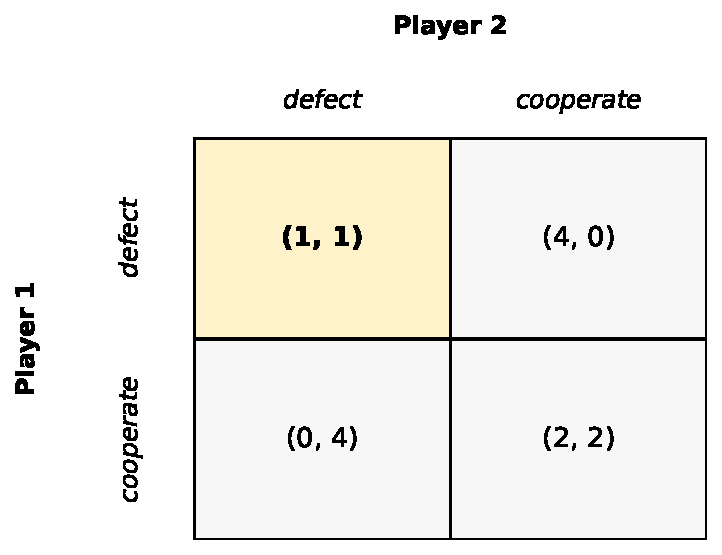
\includegraphics[width=0.42\linewidth]{payoff_pd}
  \end{center}
\end{frame}

\begin{frame}{Prisoner's Dilemma: The Nash Equilibrium}
  Ideally both players would wish to cooperate, but this creates an
  incentive for either player to defect: if the other player cooperates,
  defecting yields utility $4$ instead of $2$; if the other player
  defects, defecting still yields utility $1$ instead of $0$. Defecting is
  therefore the best response to \emph{either} of the opponent's actions,
  leading to the Nash equilibrium of (defect, defect) -- a strictly worse
  outcome for both players than (cooperate, cooperate).

  \vspace{0.4em}
  Very serious real-world versions of this dilemma are the \emph{tragedy
  of the commons} for shared physical resources, which (without global
  cooperation) leads to pollution, overfishing, and deforestation.
\end{frame}

\begin{frame}{Stag Hunt}
  Two hunters are on a hunting trip together. They may cooperate to hunt a
  \emph{stag}, or hunt \emph{alone} for a rabbit. If both hunt alone, they
  each catch and share a rabbit (utility 2). If they hunt together, they
  catch a stag and both obtain utility 4. If one hunts alone while the
  other hunts the stag, the rabbit hunter gets the rabbit to himself
  (utility 3), while the lone stag-hunter is unsuccessful (utility 0).
  \begin{center}
    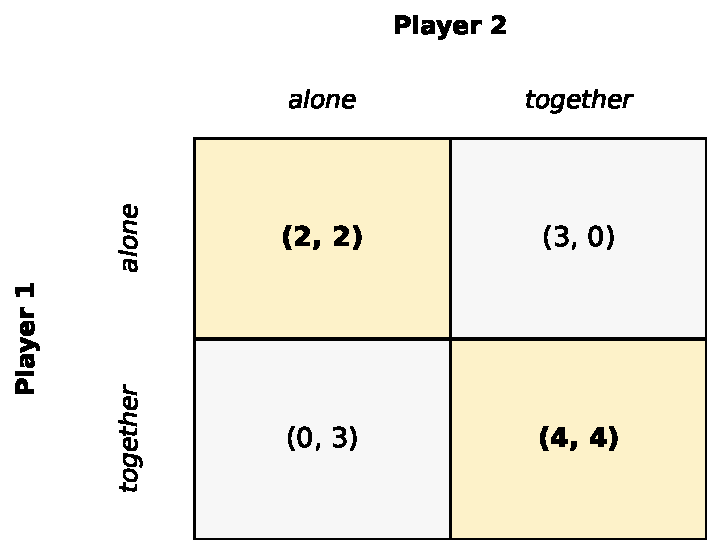
\includegraphics[width=0.42\linewidth]{payoff_sh}
  \end{center}
\end{frame}

\begin{frame}{Stag Hunt: Cooperation Is Also a Nash Equilibrium}
  Stag Hunt may look similar to the Prisoner's Dilemma, but has one key
  difference: the \emph{highest} utility for each player, (together,
  together), is \emph{also} a Nash equilibrium ((alone, alone) is a
  second, worse, Nash equilibrium). This means the players have no
  incentive to fail to work together, and it is in the best interest of
  even selfish players to cooperate.

  \vspace{0.4em}
  Other examples with the same structure: two individuals rowing a boat,
  neighbours draining a meadow, coordination of slime molds, hunting
  practices of orcas, and countries improving corporate governance
  together.
\end{frame}

\begin{frame}{Chicken}
  Two thrill-seekers play a game of brinkmanship: both drive cars toward
  each other on a head-on collision course. Either driver can
  \emph{swerve} or \emph{not swerve}. If one swerves and the other does
  not, the swerver is a ``chicken'' (utility 1) while the other gains
  admiration (utility 4). If both swerve, neither is branded a coward but
  neither gets admiration either (utility 2 each). If neither swerves,
  they crash head-on and receive utility 0 each.
  \begin{center}
    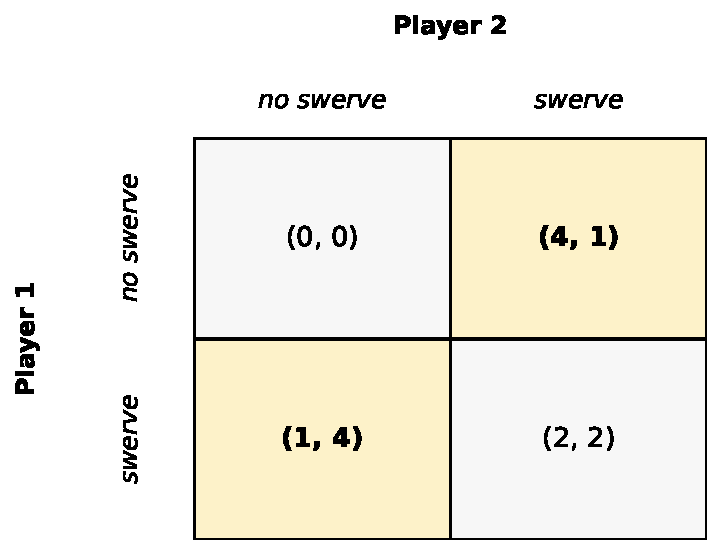
\includegraphics[width=0.42\linewidth]{payoff_chicken}
  \end{center}
\end{frame}

\begin{frame}{Chicken: Two Nash Equilibria}
  Unlike the previous two games, Chicken has \textbf{two} Nash equilibria:
  (no swerve, swerve) and (swerve, no swerve). In either case, the
  chickening player switching to not-swerving gets $0$ instead of $1$, and
  the non-swerving player switching to swerving gets $2$ instead of $4$ --
  neither wants to unilaterally deviate.

  \vspace{0.4em}
  Chicken is popular in politics, economics, and military affairs
  (achieving an advantage by pushing dangerous events to the brink),
  price wars between companies, or two people over-claiming credit for a
  joint project.
\end{frame}

\begin{frame}{Battle of the Sexes}
  A couple intends to spend an evening together. The husband prefers a
  \emph{Western}, the wife prefers a \emph{Musical}, but both would rather
  go to the \emph{same} event than different ones. Each receives utility 4
  if they attend their preferred event together, utility 2 if they attend
  the event they dislike together with their spouse, and utility 0 if they
  go separately (regardless of choice).
  \begin{center}
    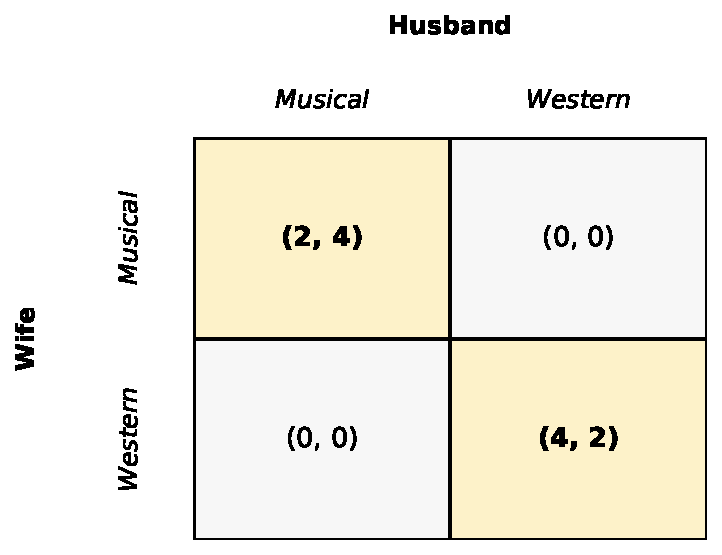
\includegraphics[width=0.42\linewidth]{payoff_bos}
  \end{center}
\end{frame}

\begin{frame}{Battle of the Sexes: Two Nash Equilibria}
  Similar to Chicken, Battle of the Sexes has two Nash equilibria:
  (Musical, Musical) and (Western, Western). However, unlike Chicken, if
  the opponent changes their action here, that will \emph{not} benefit
  you -- both equilibria are ``coordination'' outcomes, not conflicts.

  \vspace{0.4em}
  In repeated play, couples may alternate between the Musical and the
  Western -- an average utility of $3$ per game, as each player gets
  utility $4$ half the time and utility $2$ half the time (a real-life
  ``compromise''). Setting industry standards is another instance of
  Battle of the Sexes: each company prefers its in-house solution, but
  both are better off agreeing on a common standard.
\end{frame}

\begin{frame}{Matching Pennies}
  Two players each choose \emph{Heads} or \emph{Tails}. Player 1 receives
  utility 1 if both choose the \emph{same} option (0 otherwise). Player 2
  receives utility 1 if they choose \emph{different} options (0
  otherwise).
  \begin{center}
    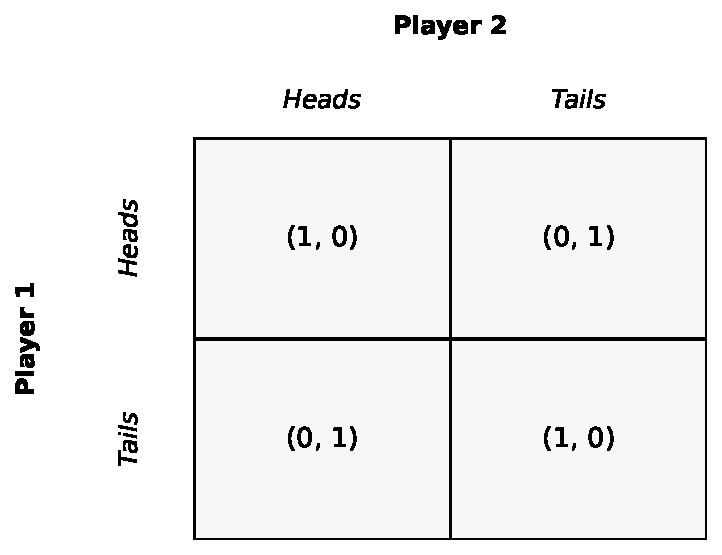
\includegraphics[width=0.42\linewidth]{payoff_mp}
  \end{center}
\end{frame}

\begin{frame}{Matching Pennies: No Pure Nash Equilibrium}
  Unlike all the previous games, Matching Pennies has \textbf{no pure
  (deterministic) Nash equilibrium}: for every action profile, the
  ``losing'' player can gain more utility by switching her strategy to the
  other action -- there is always someone who wants to deviate.

  \vspace{0.4em}
  Penalty kicks in soccer are an instance of Matching Pennies (kicker:
  left/right; goalie: jump left/right, before seeing the kick), as are
  serve-and-return plays in tennis. Rock-Paper-Scissors can be regarded as
  a three-action version of Matching Pennies.
\end{frame}

\begin{frame}[fragile]{Python: Finding Pure Nash Equilibria by Brute Force}
  We encode each game as a payoff dictionary and brute-force search all
  $4$ action profiles for Nash equilibria (Theorem 10.2.4).
  \begin{lstlisting}[style=pycode]
games = {
  "PD":  {(0,0):(1,1), (0,1):(4,0), (1,0):(0,4), (1,1):(2,2)},
  "SH":  {(0,0):(2,2), (0,1):(3,0), (1,0):(0,3), (1,1):(4,4)},
  "Chicken": {(0,0):(0,0), (0,1):(4,1), (1,0):(1,4), (1,1):(2,2)},
  "BoS": {(0,0):(2,4), (0,1):(0,0), (1,0):(0,0), (1,1):(4,2)},
  "MP":  {(0,0):(1,0), (0,1):(0,1), (1,0):(0,1), (1,1):(1,0)},
}
def is_nash(payoff, r, c):
    u1, u2 = payoff[(r, c)]
    if payoff[(1 - r, c)][0] > u1: return False  # row player deviates
    if payoff[(r, 1 - c)][1] > u2: return False  # column player deviates
    return True
for name, payoff in games.items():
    nash = [(r, c) for r in (0, 1) for c in (0, 1) if is_nash(payoff, r, c)]
    print(f"{name:9s} pure Nash equilibria: {nash}")
# PD        pure Nash equilibria: [(0, 0)]
# SH        pure Nash equilibria: [(0, 0), (1, 1)]
# Chicken   pure Nash equilibria: [(0, 1), (1, 0)]
# BoS       pure Nash equilibria: [(0, 0), (1, 1)]
# MP        pure Nash equilibria: []
  \end{lstlisting}
  This matches Theorem 10.2.4 exactly, and confirms Matching Pennies has
  no pure Nash equilibrium.
\end{frame}

\begin{frame}{10.2.4 Mixed Strategic Games}
  When acting against intelligent players in a game (especially for
  competitive games, where cooperation is not an option), we do not want
  to always deterministically choose an action, lest our opponent predicts
  our action (as in Matching Pennies, where a predictable player always
  loses). This leads us to \textbf{mixed strategic games}: instead of
  choosing an action deterministically, each player chooses a
  \textbf{probability distribution} over the set of actions, then samples
  an action according to that distribution.

  \begin{block}{Definition 10.2.9 (Mixed strategic games in normal form)}
    The \emph{mixed extension} of the strategic game
    $\langle N,(\Ac_i),(u_i)\rangle$ is the strategic game
    $\langle N,(\Delta\Ac_i),(U_i)\rangle$, where $\Delta\Ac_i$ is the set
    of all probability distributions over $\Ac_i$, and
    $U_i:\times_{j\in N}\Delta\Ac_j\to\R$ is defined as the expected value
    of $u_i$, assuming player $i$ samples his action from $\Ac_i$
    according to the distribution $\alpha_i$. Writing
    $\alpha:=(\alpha_1,\ldots,\alpha_N)$, we can express $U_i$ as
    \[
      U_i(\alpha) \;:=\; \sum_{a\in\Ac} u_i(a)\prod_{j\in N}\alpha_j(a_j)
    \]
  \end{block}
  \textbf{Plain English.} $U_i(\alpha)$ is the average payoff to player
  $i$ when every player independently samples an action from their own
  distribution $\alpha_j$; $\prod_{j\in N}\alpha_j(a_j)$ is the probability
  of the specific joint profile $a$ occurring under independent sampling.
\end{frame}

\begin{frame}{Definition 10.2.10 and Theorem 10.2.11: Mixed Nash}
  We call a distribution in $\Delta\Ac_i$ a \textbf{mixed strategy} for
  player $i$. A \emph{pure strategy} is the special case of a mixed
  strategy that is deterministic (assigns probability 1 to one action, 0
  to the rest).

  \begin{block}{Definition 10.2.10 (Mixed Nash equilibrium)}
    A \emph{mixed strategy Nash equilibrium} of a strategic game is a
    Nash equilibrium of the mixed extension: a collection
    $\alpha^*=(\alpha_1^*,\ldots,\alpha_N^*)$ such that each
    $\alpha_i^*\in\Delta\Ac_i$, and no player would gain more (expected)
    utility by choosing a different distribution: for all players $i$ and
    all $\alpha_i\in\Delta\Ac_i$,
    \[
      U_i(\alpha^*) \;\geq\; U_i(\alpha^*_{\neq i},\alpha_i)
    \]
  \end{block}
  Every ordinary (pure) Nash equilibrium $a^*$ is a special case of a
  mixed Nash equilibrium, obtained via $\alpha_i^*(x)=[\![x=a_i^*]\!]$.

  \begin{block}{Theorem 10.2.11 (Existence of mixed Nash equilibrium)}
    Every finite strategic game has a mixed strategy Nash equilibrium.
  \end{block}
  \textbf{Proof sketch.} Identify $\Delta\Ac_i$ with the probability
  simplex $\{(p_1,\ldots,p_{m_i}):p_j\geq0,\sum_j p_j=1\}$, where
  $m_i:=|\Ac_i|$. This set is nonempty, convex, and compact. Since
  expectations are linear, one can define $a\succeq_i b$ iff
  $U_i(a)\geq U_i(b)$, which satisfies the premises of Theorem 10.2.7 for
  the mixed extension. $\blacksquare$
\end{frame}

\begin{frame}{Finding the Mixed Nash Equilibrium of Matching Pennies}
  Recall that Matching Pennies has \emph{no} pure Nash equilibrium.
  However, since the game is finite, Theorem 10.2.11 guarantees a mixed
  Nash equilibrium exists.

  \vspace{0.3em}
  If Player 1 chooses (Heads, Tails) with probabilities
  $(\tfrac12,\tfrac12)$, then the expected utility for both players is
  $\tfrac12$, regardless of what strategy the opponent chooses -- mixed or
  otherwise. Hence, if both players choose the mixed strategy
  $(\tfrac12,\tfrac12)$, neither has an incentive to switch to any other
  mixed strategy (all mixtures are equally good against a uniformly
  random opponent), so both players choosing $(\tfrac12,\tfrac12)$ is a
  mixed Nash equilibrium.

  \vspace{0.3em}
  In fact, it is the \emph{only} such equilibrium. If Player 1 chose some
  other mixed strategy $(\theta,1-\theta)$ with $\theta\neq\tfrac12$, then
  Player 2 would choose a deterministic strategy of always Heads
  ($\theta<\tfrac12$) or always Tails ($\theta>\tfrac12$) -- giving Player
  2 expected utility $\max\{\theta,1-\theta\}>\tfrac12$. The same argument
  applies to Player 1 if Player 2 deviates from $(\tfrac12,\tfrac12)$.
\end{frame}

\begin{frame}{Matching Pennies: Visualizing the Mixed Nash Equilibrium}
  The plot below shows Player 2's expected utility from playing Heads
  versus Tails, as a function of $\theta$ (Player 1's probability of
  playing Heads). The two lines cross exactly at $\theta=\tfrac12$, which
  is where neither of Player 2's pure actions is strictly better than the
  other -- confirming that $(\tfrac12,\tfrac12)$ is the mixed Nash
  equilibrium.
  \begin{center}
    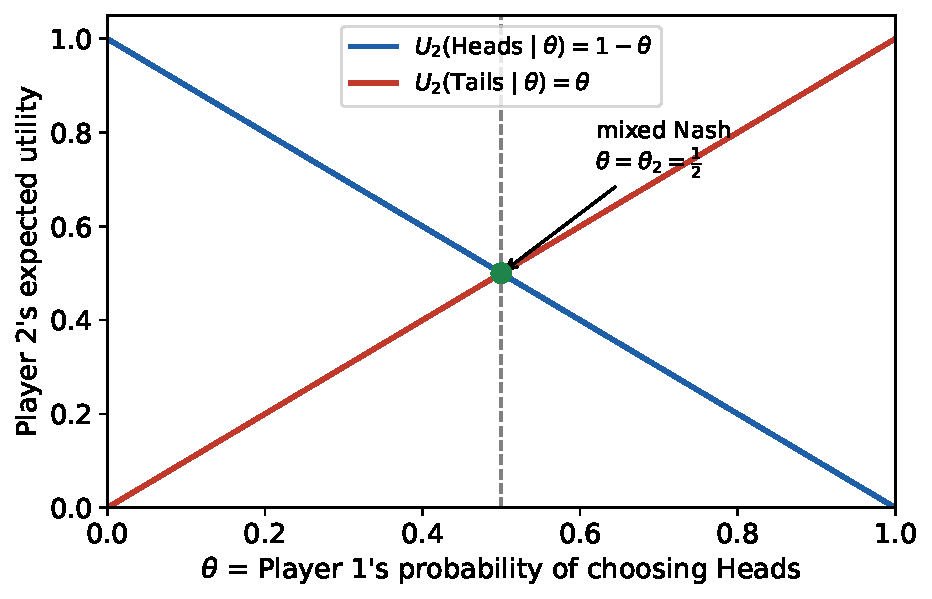
\includegraphics[width=0.62\linewidth]{mixed_nash_mp}
  \end{center}
\end{frame}

\begin{frame}[fragile]{Python: Verifying the Mixed Nash Equilibrium of Matching Pennies}
  We numerically check that Player 2's expected utility is maximized at
  $\theta=\tfrac12$ (Player 1's probability of Heads), confirming no
  profitable deviation exists at the symmetric mixture.
  \begin{lstlisting}[style=pycode]
def u2_expected(theta, p2_heads):
    # Player 2 gets utility 1 iff actions differ.
    # theta = P(P1=Heads); p2_heads = P(P2=Heads)
    p_diff = theta * (1 - p2_heads) + (1 - theta) * p2_heads
    return p_diff

theta = 0.5
for p2_heads in [0.0, 0.25, 0.5, 0.75, 1.0]:
    print(f"P2 plays Heads w.p. {p2_heads:.2f} -> "
          f"U2 = {u2_expected(theta, p2_heads):.3f}")

# P2 plays Heads w.p. 0.00 -> U2 = 0.500
# P2 plays Heads w.p. 0.25 -> U2 = 0.500
# P2 plays Heads w.p. 0.50 -> U2 = 0.500   (all mixtures tie: theta=1/2 is Nash)
# P2 plays Heads w.p. 0.75 -> U2 = 0.500
# P2 plays Heads w.p. 1.00 -> U2 = 0.500

theta = 0.7   # if Player 1 deviates from 1/2 ...
best = max(u2_expected(theta, p) for p in [0.0, 1.0])
print(f"theta=0.7: best pure response for P2 gives U2={best:.3f} > 0.5")
# theta=0.7: best pure response for P2 gives U2=0.700 > 0.5   (P2 deviates!)
  \end{lstlisting}
\end{frame}

%% ══════════════════════════════════════════════════════════════════════════
\section{10.3 Multi-Agent Extensive-Form Games}

\begin{frame}{From One-Shot to Multi-Round Games}
  As currently defined, a strategic game has a \emph{single round} of
  interaction. More interesting are games where all players choose an
  action (or an action is sampled from a chosen distribution), the
  players' actions are revealed, players receive utility according to the
  utility functions, and then players choose an action again for the next
  round, using the previous history of action profiles and received
  utilities as a guide. Multi-round strategic games are called
  \textbf{extensive-form games}.

  \vspace{0.4em}
  This setting is extremely general -- much more general than repeated
  (i.i.d.) matrix games. It generalizes the history-based (essentially
  assumption-free) reinforcement learning setting to modelling multiple
  agents, with simultaneous or sequential actions.
\end{frame}

\begin{frame}{Figure 10.1: Agents in a Multi-Agent Environment}
  \begin{center}
    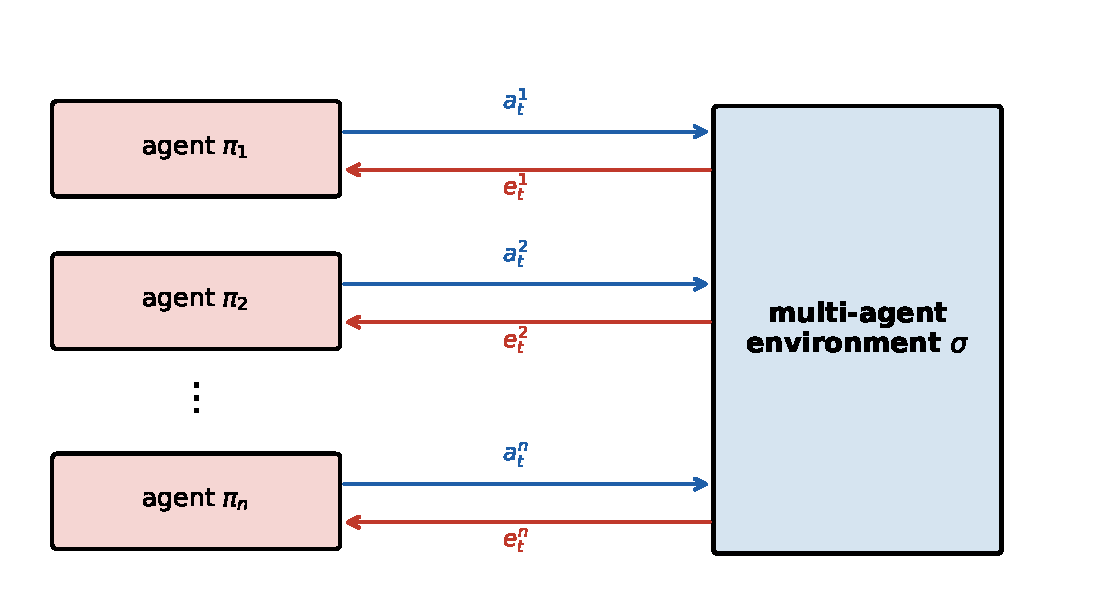
\includegraphics[width=0.68\linewidth]{multi_agent_diagram}
  \end{center}
  \textbf{Figure 10.1.} Agents $\pi_1,\ldots,\pi_n$ (each $\pi_i$, ``pi
  sub $i$'', is agent $i$'s policy) interact with a shared multi-agent
  environment $\sigma$ (``sigma''), each only seeing its \emph{own} action
  $a_t^i$ and \emph{own} percept $e_t^i$ at every time step $t$.
\end{frame}

\begin{frame}{Formalizing the Multi-Agent Environment}
  In an extensive-form game / multi-agent setting there are $n$ agents,
  each taking actions sequentially from the finite action space $\Ac$. At
  each time step $t=1,2,\ldots$, the environment receives an action
  $a_t^i$ from agent $i$ and outputs $n$ percepts
  $e_t^1,\ldots,e_t^n\in\Ec$, one for each agent. Each percept
  $e_t^i=(o_t^i,r_t^i)$ contains an observation $o_t^i$ and a reward
  $r_t^i\in[0,1]$. Importantly, agent $i$ only sees its own action $a_t^i$
  and its own percept $e_t^i$ (Figure 10.1).

  \vspace{0.3em}
  \textbf{Shorthand notation.} We write $a_t:=(a_t^1,\ldots,a_t^n)$ and
  $e_t:=(e_t^1,\ldots,e_t^n)$ for the joint action/percept at time $t$,
  and denote $h_{<t}^i=a_1^ie_1^i\ldots a_{t-1}^ie_{t-1}^i$ (agent $i$'s
  own history) and $h_{<t}=a_1e_1\ldots a_{t-1}e_{t-1}$ (the full joint
  history).

  \vspace{0.3em}
  We define a \textbf{multi-agent environment} as a probability kernel
  \[
    \sigma:(\Ac^n\times\Ec^n)^*\times\Ac^n \to \Delta(\Ec^n)
  \]
  \textbf{Plain English.} Given the full history so far and the joint
  action just taken by all $n$ agents, $\sigma$ returns a probability
  distribution over the joint percept $(e_t^1,\ldots,e_t^n)$ that all
  agents will receive next.
\end{frame}

\begin{frame}{The History Distribution}
  The $n$ agents are given by $n$ policies $\pi_1,\ldots,\pi_n$, where
  $\pi_i:(\Ac\times\Ec)^*\to\Delta\Ac$ (each agent's policy maps its own
  history to a distribution over its next action). Together, the policies
  and the environment specify the \textbf{history distribution}
  \begin{align*}
    \sigma^{\pi_{1:n}}(\epsilon) &:= 1 \\
    \sigma^{\pi_{1:n}}(h_{1:t}) &:= \sigma^{\pi_{1:n}}(h_{<t}a_t)\,\sigma(e_t\mid h_{<t}a_t) \\
    \sigma^{\pi_{1:n}}(h_{<t}a_t) &:= \sigma^{\pi_{1:n}}(h_{<t})\prod_{i=1}^n \pi_i(a_t^i\mid h_{<t}^i)
  \end{align*}
  \textbf{Plain English.} The probability of the empty history is $1$
  (line 1). The probability of a history extended by one more joint
  percept $e_t$ (line 2) is the probability of everything up to and
  including the joint action $a_t$, times the environment's chance of
  producing $e_t$ given that action. The probability of extending a
  history by a joint action $a_t$ (line 3) is the probability of the
  history so far, times the product over all $n$ agents of the chance
  \emph{that agent} takes the action it took, based only on \emph{its own}
  history $h_{<t}^i$ -- capturing that each agent decides independently,
  using only what it personally has observed.
\end{frame}

\begin{frame}{Definition 10.3.1: Multi-Agent $\varepsilon$-Best Response}
  Our definition of a multi-agent environment is very general and
  encompasses most of game theory: it allows for cooperative,
  competitive, and mixed games; infinitely repeated games; or any
  (infinite-length) extensive-form game with finitely many players.

  \begin{block}{Definition 10.3.1 (Multi-agent $\varepsilon$-best response and $\varepsilon$-Nash equilibrium)}
    The policy $\pi_i$ is an $\varepsilon$-\emph{best response}
    ($\varepsilon$, ``epsilon'', a small positive tolerance) after history
    $h_{<t}^i$ iff
    \[
      V^*_{\sigma_i}(h^i_{<t}) - V^{\pi_i}_{\sigma_i}(h^i_{<t}) \;<\; \varepsilon
    \]
    If at some time step $t$, all agents' policies are $\varepsilon$-best
    responses, we have an $\varepsilon$-\emph{Nash equilibrium}.
  \end{block}
  \textbf{Plain English.} $V^*_{\sigma_i}$ is the best possible value
  (expected future reward) agent $i$ could achieve in its own
  \textbf{subjective environment} $\sigma_i$ (defined next section), and
  $V^{\pi_i}_{\sigma_i}$ is the value it actually achieves by following
  $\pi_i$. If the gap between the two is less than $\varepsilon$ for every
  agent simultaneously, no agent is leaving more than $\varepsilon$ worth
  of value on the table -- an approximate, ``fuzzy'' Nash equilibrium. The
  property of multi-agent systems analogous to \emph{asymptotic
  optimality} (Chapters 8--9) is convergence to an $\varepsilon$-Nash
  equilibrium.
\end{frame}

%% ══════════════════════════════════════════════════════════════════════════
\section{10.4 Strategic Games vs Reinforcement Learning}

\begin{frame}{A Terminology Dictionary}
  There are a lot of immediate similarities between strategic games and
  the sequential decision theory / (history-based) reinforcement learning
  setup from earlier chapters. Both have a set of actions an agent can
  take, and both have some sort of reward or utility that the agent wants
  to maximize.

  \begin{center}
  \begin{tabular}{r c l}
    \toprule
    \textbf{Reinforcement learning} & $=$ & \textbf{Game theory} \\
    \midrule
    stochastic policy & $=$ & mixed strategy \\
    deterministic policy & $=$ & pure strategy \\
    agent & $=$ & player \\
    multi-agent environment & $=$ & infinite extensive-form game \\
    value & $=$ & payoff/utility \\
    (finite) history & $=$ & history \\
    infinite history & $=$ & path of play \\
    \midrule
    asymptotic optimality & $=$ & convergence to Nash \\
    \bottomrule
  \end{tabular}
  \end{center}
  \textbf{Table 10.2.} Terminology dictionary between reinforcement
  learning and extensive-form game theory {\footnotesize[LTF16]}.
\end{frame}

\begin{frame}{The Subjective Environment $\sigma_i$}
  Each agent $i$ acts in a \textbf{subjective environment} $\sigma_i$,
  obtained by joining the multi-agent environment $\sigma$ with the
  policies $\pi_1,\ldots,\pi_{i-1},\pi_{i+1},\ldots,\pi_n$ of everyone
  \emph{else}, by marginalizing (summing) over the histories that $\pi_i$
  does not see. Together with policy $\pi_i$, the environment $\sigma_i$
  yields a distribution over the histories of agent $i$:
  \[
    \sigma_i^{\pi_i}(h_{<t}^i) \;:=\; \sum_{h'_{<t},\,j\neq i} \sigma^{\pi_{1:n}}(h_{<t})
  \]
  \textbf{Plain English.} We obtain agent $i$'s subjective, single-agent
  view of the world by averaging away (marginalizing over) all the
  possible histories $h'_{<t}$ that the \emph{other} agents $j\neq i$
  could have experienced, weighted by how likely each is under the full
  joint history distribution.

  \vspace{0.3em}
  It is crucial to note that the subjective environment $\sigma_i$ and the
  policy $\pi_i$ are \emph{ordinary} (single-agent) environments and
  policies, so we can use the history-based RL formalism from Chapters 6
  and 7. Furthermore, we can interpret policy $\pi_i$ as a (one-shot)
  mixed strategy $\alpha_i$ of player/agent $i$, and the value
  $V^{\pi_i}_{\sigma_i}(\epsilon)$ as their utility $U_i(\alpha)$ -- this
  reduces the extensive-form game to a normal-form game, so many results
  for the latter apply here too.
\end{frame}

\begin{frame}{From Strategic Games to Reinforcement Learning}
  We can convert any extensive-form strategic game into the reinforcement
  learning setting: let the actions in the game be the actions of the
  agent, and the utilities $U_i(\alpha)$ be the value $V^{\pi_i}_{\sigma_i}$.
  The agent represents one of the players, and the environment simulates
  the actions of all other players.

  \vspace{0.3em}
  However simple this conversion sounds, it misses the point of strategic
  games: modelling the actions of an \emph{intelligent adversary}, or
  learning to cooperate/compromise so both players benefit. In classical
  MDP reinforcement learning this is rarely captured, since results
  typically assume \emph{stationary} environments (the strategy of all
  other players is fixed) -- meaning the opponents cannot learn or adapt
  when they are being exploited.

  \vspace{0.3em}
  This is not to say \emph{all} RL lacks intelligent adversaries:
  Backgammon {\footnotesize[Tes94]}, Go {\footnotesize[SH+16]}, and
  StarCraft {\footnotesize[VBC+19]} are interesting precisely because of
  the intelligent adversary. Often such environments can be represented
  as zero-sum games, with the opponent's reward as the negative of the
  agent's.

  \vspace{0.3em}
  \textbf{Why this matters for AIXI.} AIXI assumes the true environment
  lies within its Bayesian mixture class $\Mc_{sol}$. This assumption may
  hold for simple strategic games, but \emph{fails} if AIXI were to play
  against itself (or another AIXI-like agent) -- a reflective problem
  addressed in the remaining sections of this chapter.
\end{frame}

\begin{frame}{From Reinforcement Learning to Strategic Games}
  This transformation can also be \textbf{reversed}: by keeping the
  agent's action space as it was in the RL setting, we represent each
  state or observation of the environment as an action taken by the
  ``opponent''. The agent receives a payoff equal to the reward for every
  action-state pair, and the opponent receives the agent's negative
  payoff.

  \vspace{0.3em}
  \textbf{A notable limitation.} The strategic game's ``opponent'' may not
  aim for optimal actions, since the environment selects actions based on
  its own distribution. This contradicts one of game theory's core
  principles: that all players strive for optimal performance. Setting
  the opponent's payoff matrix to identically zero does not help either:
  \emph{any} best response strategy of the agent to \emph{any} strategy of
  the opponent is then trivially a Nash equilibrium.

  \vspace{0.3em}
  Regardless, various aspects of reinforcement learning can be adapted to
  the strategic game framework:
  \begin{itemize}
    \item MDPs can be represented by \textbf{Markov opponents}.
    \item Partially observable environments can be mirrored by
      \textbf{partially observable opponent actions}.
    \item Computable environments can be incorporated by ensuring the
      game and its opponents are \textbf{computable}.
  \end{itemize}
\end{frame}

%% ══════════════════════════════════════════════════════════════════════════
\section{10.5 Reflective Oracles}

\begin{frame}{The Self-Modelling Problem}
  In computational game theory, we can model players as agents running on
  Turing machines. In this setup, how will two \emph{optimal} agents act
  if they know the other agent's code, and both know they have the code of
  the other, etc? Naively, each agent will run the other agent's program,
  which will run their own program, which will run the other agent's
  program, and so on -- an infinite regress.

  \vspace{0.3em}
  One fix is to only run this recursion a fixed number of times -- but
  what if the opponent recurses \emph{more}? To overcome this
  self-modelling problem, {\footnotesize[FTC15]} introduced a probabilistic
  oracle called a \textbf{Reflective Oracle}: a truly remarkable
  construction. When an agent is run with a Reflective Oracle, it is able
  to reason about itself and overcome the self-modelling problem.
\end{frame}

\begin{frame}{Probabilistic Turing Machines and Semimeasures}
  Let $\Tc$ denote the set of \textbf{probabilistic Turing machines}. Each
  $T\in\Tc$ corresponds to a conditional semimeasure $\nu_T$ (``nu sub
  $T$''), where $\nu_T(a\mid x)$ is the probability that $T$ outputs
  $a\in\B$ given input $x\in\B^*$ ($\B$ = the set of finite/infinite bit
  strings). Note that $\sum_{a\in\B}\nu_T(a\mid x)$ may be smaller than
  $1$, since $T$ may not halt. We can define $\nu_T(x)$ via the chain
  rule,
  \[
    \nu_T(x) \;:=\; \prod_{k=1}^{\ell(x)} \nu_T(x_k\mid x_{<k})
  \]
  which is \textbf{lower semicomputable} (we can approximate it from
  below, getting arbitrarily close but never overshooting, in finite
  time), since each factor is lower semicomputable. This construction
  differs from a general solomonoff semimeasure $\nu\in\Mc_{sol}$, since
  for a general $\nu$, the predictive distribution $\nu(a\mid x)$ may not
  be lower semicomputable.

  \vspace{0.3em}
  \textbf{Oracles.} An \emph{oracle} is a function which gives access to
  information that would otherwise be hard or impossible to compute. The
  oracle receives a question (a \emph{query}) and provides a yes or no
  answer. A well-known example is the (incomputable) \textbf{Halting
  oracle}: it takes an (encoded) machine-input pair $\langle T,x\rangle$
  and returns \emph{Yes} if machine $T$ halts on input $x$, and \emph{No}
  otherwise.
\end{frame}

\begin{frame}{Oracle Machines}
  We extend Turing machines and Turing computability to include oracles.
  Let $T^O$ denote a Turing machine $T\in\Tc$ with access to oracle $O$:
  that is, $T^O$ is an \textbf{oracle machine}, an extended (probabilistic)
  Turing machine that additionally has an oracle tape and oracle head used
  to query the oracle and write back $1=$Yes or $0=$No (counted as only
  one time step) {\footnotesize[RJ87]}. For instance, if $O$ is the
  Halting oracle, $T^O$ now has the power to solve the halting problem. Of
  course, due to the \textbf{Church--Turing thesis} (Thesis 2.6.6), no
  real computer can compute $T^O$ for incomputable oracles $O$. Let
  $\nu_T^O$ denote the semimeasure induced by $T^O$.

  \vspace{0.3em}
  The oracles $O:\Tc\times\B^*\times\mathbb{Q}\to\Delta\B$ we consider
  take as input (an encoding of) a Turing machine and an input on that
  Turing machine, as well as a rational number, and return a (possibly
  randomized) $\text{Yes}=1$ or $\text{No}=0$ based on this input.

  \vspace{0.3em}
  \textbf{The specific oracle we consider} has the following property:
  each oracle takes a query $\langle T,x,z\rangle$ -- a Turing machine $T$,
  an input $x$ to $T$, and a rational number $z$ -- and returns $1$ if the
  probability that $T^O$ outputs $1$ on input $x$ is greater than $z$,
  that is, for the induced semimeasure $\nu_T^O(1\mid x)>z$. It returns
  $0$ if $\nu_T^O(0\mid x)>1-z$. If neither is satisfied, the oracle may
  return $0$ or $1$ randomly, as it pleases.
\end{frame}

\begin{frame}{Definition 10.5.1: Reflective Oracle}
  \begin{block}{Definition 10.5.1 (Reflective Oracle)}
    An oracle $O:\Tc\times\B^*\times\mathbb{Q}\to\Delta\B$ is
    \emph{reflective} if and only if for all queries
    $(T,x,z)\in\Tc\times\B^*\times\mathbb{Q}$,
    \begin{itemize}
      \item If $\nu_T^O(1\mid x) > z$ then $O(T,x,z)=1$,
      \item If $\nu_T^O(0\mid x) > 1-z$ then $O(T,x,z)=0$,
      \item Else $O(T,x,z)$ may return $0$ or $1$ at random (with any
        probability).
    \end{itemize}
  \end{block}
  \textbf{Plain English.} The oracle must be \emph{consistent} about
  itself: since the queried machine $T$ may itself query the oracle $O$
  (possibly about itself, or about other machines that query $O$, and so
  on), the oracle's answers must be compatible with the very semimeasure
  they help define -- hence the name \emph{reflective}.
\end{frame}

\begin{frame}{Visualizing the Reflective Oracle}
  The reflective oracle lets a Turing machine $T^O$ query information
  about a semimeasure -- including possibly \emph{about itself} -- while
  guaranteeing the answers stay logically consistent.
  \begin{center}
    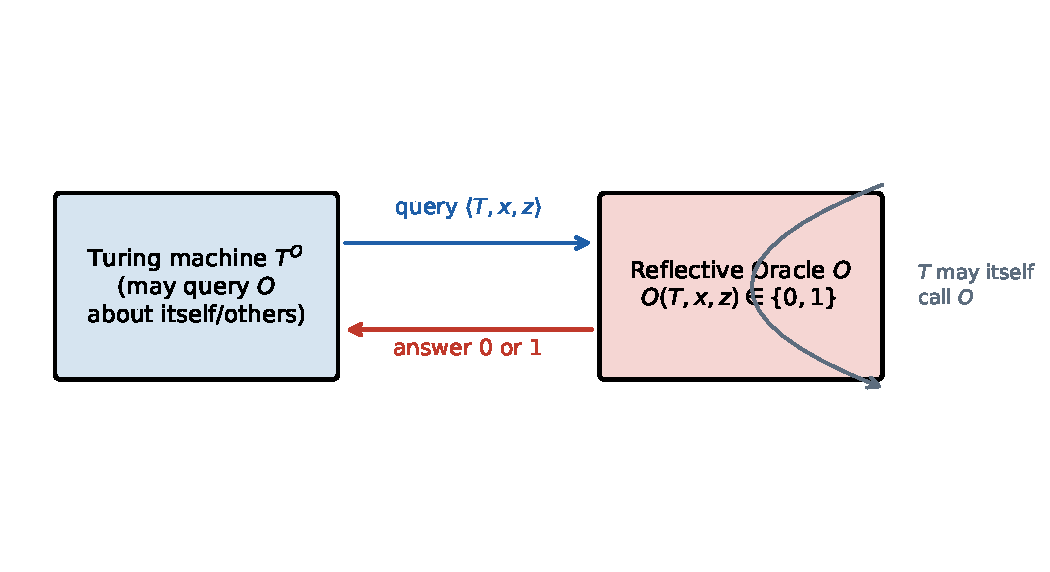
\includegraphics[width=0.58\linewidth]{reflective_oracle_schematic}
  \end{center}
  The machine $T^O$ sends a query $\langle T,x,z\rangle$; the oracle $O$
  answers $0$ or $1$ following Definition 10.5.1's three cases. Since $T$
  may itself contain calls to $O$, the oracle's answer must remain
  consistent under this self-reference -- the defining challenge that
  makes reflective oracles remarkable.
\end{frame}

\begin{frame}{Definition 10.5.2 and the Normalization Formula (10.5.3)}
  \begin{block}{Definition 10.5.2 (Reflective-oracle-computable)}
    A semimeasure is \emph{reflective-oracle-computable} if and only if it
    is computable on a probabilistic Turing machine with access to a
    Reflective Oracle. That is, there exists a probabilistic Turing
    machine $T$ and Reflective Oracle $O$ such that the semimeasure can be
    computed with $T^O$.
  \end{block}
  Recall that \emph{normalizing} a semimeasure $\nu$ means increasing it
  to a measure $\bar\nu$ such that $\nu(0\mid x)+\nu(1\mid x)=1$. We can
  normalize the Reflective Oracle semimeasure $\nu_T^O$ for any
  probabilistic Turing machine $T$, giving a Reflective Oracle
  \emph{measure} $\bar\nu_T^O$, using binary search with the oracle $O$ to
  find the \emph{crossover point} $z^*\in[0,1]$ where $O(T,x,z)$ changes
  from returning $1$ to $0$, i.e.\ $\nu_T^O(1\mid x)\leq z^*\leq
  1-\nu_T^O(0\mid x)$. If $\nu_T^O(1\mid x)+\nu_T^O(0\mid x)<1$, $z^*$ may
  be random, so we take the expectation:
  \[
    \bar\nu_T^O(1\mid x) \;:=\; \E[z^*\mid x,\nu_T^O] \;=:\; 1-\bar\nu_T^O(0\mid x) \quad\text{for all }x \tag{10.5.3}
  \]
  By construction, $\bar\nu_T^O(a\mid x)$ is a reflective-oracle-computable
  (properly normalized) measure, and $\bar\nu_T^O(a\mid x)\geq\nu_T^O(a\mid x)$.
\end{frame}

\begin{frame}{Theorem 10.5.4: Existence of a Reflective Oracle}
  It is far from obvious whether Reflective Oracles even exist, and if so,
  whether they are reasonably computable. Remarkably, both questions have
  the answer: yes.
  \begin{block}{Theorem 10.5.4 (Existence of a limit-computable Reflective Oracle {\footnotesize[LTF16]})}
    There exists a limit-computable (Definition 2.6.13) Reflective Oracle.
  \end{block}
  \textbf{Plain English.} A \textbf{limit-computable} function is one for
  which there is a computable sequence of guesses that eventually
  converges to (``settles on'') the true value, even though we may never
  know \emph{when} it has converged. This is weaker than ordinary
  computability, but very low in the arithmetic hierarchy ($\Delta_2^0$,
  Definition 2.6.17).

  \vspace{0.3em}
  The proof requires constructing an infinite hierarchy of partially
  reflective partial oracles and is beyond the scope of the book
  {\footnotesize[LTF16]}. One can also show that Reflective Oracles are
  \emph{not} Halting Oracles (due to their randomization), and that they
  are not computable.
\end{frame}

\begin{frame}[fragile]{Python: Simulating a Reflective Oracle's Decision Rule}
  We cannot literally compute an incomputable oracle, but we can simulate
  Definition 10.5.1's three-way decision rule for a toy machine $T$ whose
  true output-1 probability $p=\nu_T^O(1\mid x)$ is known to us (the
  simulator), for several queried thresholds $z$.
  \begin{lstlisting}[style=pycode]
import random
random.seed(0)

def reflective_oracle_query(p, z):
    """p = true P(T outputs 1 | x); z = queried threshold."""
    if p > z:
        return 1                      # nu_T^O(1|x) > z
    elif (1 - p) > (1 - z):            # nu_T^O(0|x) > 1-z
        return 0
    else:
        return random.choice([0, 1])  # free choice region

p = 0.62  # true probability that T outputs 1
for z in [0.10, 0.40, 0.62, 0.80, 0.95]:
    outcome = reflective_oracle_query(p, z)
    print(f"query z={z:.2f}: O(T,x,z) = {outcome}")

# query z=0.10: O(T,x,z) = 1     (p=0.62 > z=0.10)
# query z=0.40: O(T,x,z) = 1     (p=0.62 > z=0.40)
# query z=0.62: O(T,x,z) = 0 or 1  (tie: free-choice region, p==z)
# query z=0.80: O(T,x,z) = 0     ((1-p)=0.38 > 1-z=0.20)
# query z=0.95: O(T,x,z) = 0     ((1-p)=0.38 > 1-z=0.05)
  \end{lstlisting}
  Binary-searching over $z$ this way is exactly how (10.5.3) locates the
  crossover point $z^*\approx p$ to normalize $\nu_T^O$.
\end{frame}

%% ══════════════════════════════════════════════════════════════════════════
\section{10.6 The Grain of Truth}

\begin{frame}{The Grain of Truth Problem}
  When an agent is in a multi-agent setting, and each agent believes that
  every other agent is acting optimally, what should each agent do? This
  is the \textbf{Grain of Truth} problem. Each agent models the behaviour
  of the opposing agents, and each of these opposing agents is modelling
  the behaviour of the agent, which includes models of the opposing
  agents, and so on. This can go on forever, or up to the maximum depth
  allowed by each agent.

  \vspace{0.4em}
  The Grain of Truth problem is finding \emph{when} this chain of beliefs
  about opponents' beliefs about itself has a solution. To solve it, we
  take a \textbf{Bayesian} approach.
\end{frame}

\begin{frame}{Visualizing the Infinite Regress}
  \begin{center}
    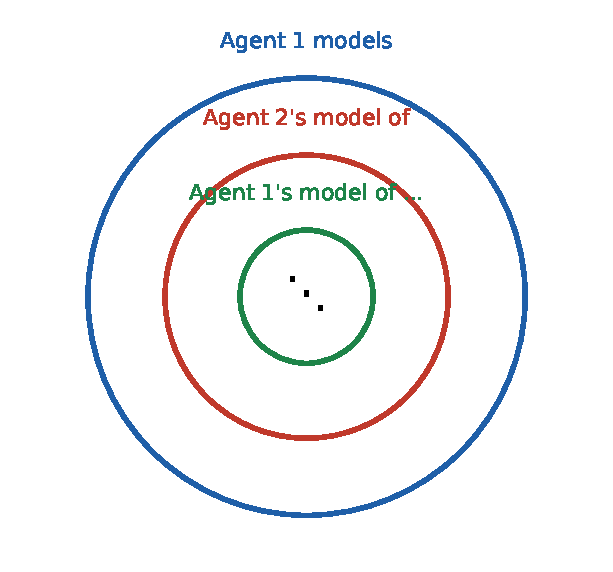
\includegraphics[width=0.42\linewidth]{grain_of_truth_schematic}
  \end{center}
  Agent 1 models the environment, which includes Agent 2. Agent 2's model
  of Agent 1 in turn contains a model of Agent 1's model of Agent 2, and
  so on -- an infinite nested regress of ``models of models''. The Grain
  of Truth problem asks when this infinite chain is well defined and
  contains a grain (a small but nonzero piece) of the truth needed for
  learning to work.
\end{frame}

\begin{frame}{Strategy: Solving Grain of Truth with Reflective Oracles}
  In this section we show how Reflective Oracles can be used to solve the
  Grain of Truth problem, in three steps:
  \begin{enumerate}
    \item Define a class of environments $\Mc$.
    \item Show that the Bayesian mixture over $\Mc$ is itself contained
      \emph{within} the class $\Mc$.
    \item Show that the optimal policy over this class is Reflective
      Oracle computable.
  \end{enumerate}
  Formally, the Grain of Truth problem entails identifying a collection of
  environments $\Mc$ such that the optimal policy $\pi^*_{\xi_\Mc}$
  derived from the Bayesian mixture $\xi_\Mc$ over $\Mc$ itself belongs to
  $\Mc$. It is crucial that $\Mc$ represents a class encompassing
  \emph{both} policies and environments simultaneously, since we are
  examining a multi-agent setting where the environment is also
  considered an (opponent) policy.

  \vspace{0.3em}
  Reflective Oracles have so far only been developed for binary sequences.
  This is not a problem, because we can bijectively map actions and
  observations to binary complete prefix codes
  {\footnotesize[MH21b, CHV22a, MH21a]}, and take products of conditional
  binary predictive distributions, which we henceforth assume.
\end{frame}

\begin{frame}{Definition 10.6.1: Reflective Environments}
  \begin{block}{Definition 10.6.1 (Reflective environments)}
    The class of \emph{reflective environments} with respect to a set of
    Turing machines $\Tc$ and a fixed reflective oracle $O$ is defined by
    \[
      \Mc_r^O \;:=\; \{\bar\nu_T^O : T\in\Tc\} \qquad\text{(see (10.5.3))}
    \]
  \end{block}
  Recall the definition of a Bayesian mixture (Definitions 7.2.1 and
  7.2.2), this time over $\Mc_r^O$:
  \[
    \xi(e_t\mid h_{<t}a_t) \;:=\; \sum_{\nu\in\Mc_r^O} w(\nu\mid h_{<t})\,\nu(e_t\mid h_{<t}a_t)
  \]
  but with one key difference: $w(\nu\mid h_{<t})$ is the recursively
  defined \emph{renormalized posterior},
  \[
    w(\nu\mid h_{1:t}) \;:=\; w(\nu\mid h_{<t})\,\frac{\nu(e_t\mid h_{<t}a_t)}{\bar\xi(e_t\mid h_{<t}a_t)}
  \]
  We can choose any lower semicomputable prior, e.g.\
  $w_{\bar\nu_T^O}=2^{-K(T)}$, in line with AIXI, where $K$ is the
  Kolmogorov complexity (Section 2.7).
\end{frame}

\begin{frame}{Theorem 10.6.2: Bayes Is a Reflective Environment}
  \begin{block}{Theorem 10.6.2 (Bayes is a reflective environment {\footnotesize[Lei16b]})}
    The Bayesian normalized mixture $\bar\xi$ is an element of $\Mc_r^O$,
    that is, $\bar\xi\in\Mc_r^O$.
  \end{block}
  \textbf{Why this matters.} This is the crucial step: it says the
  Bayes-optimal environment (the ``average'' over everything the agent
  currently believes) is \emph{itself} a valid member of the very class
  $\Mc_r^O$ it was built from -- exactly the self-consistency the Grain of
  Truth problem demands.

  \vspace{0.3em}
  \textbf{Proof sketch.} By induction over $t$, it is easy to see that
  $\xi$ is reflective-oracle-lower-semicomputable. Assume $w(\nu\mid
  h_{<t})$ is reflective-oracle-lower-semicomputable, which is true for
  $t=1$. This implies $\xi(e_t\mid h_{<t}a_t)$ is
  reflective-oracle-lower-semicomputable. Hence there exists an oracle
  machine $T'$ such that $\xi(e_t\mid h_{<t}a_t)=\nu_{T'}^O(e_t\mid
  h_{<t}a_t)$, hence the normalized $\bar\xi(e_t\mid
  h_{<t}a_t)=\bar\nu_{T'}^O(e_t\mid h_{<t}a_t)$ is
  reflective-oracle-computable. This normalization is the key difference
  from Definition 7.2.2, and makes the posterior $w(\nu\mid h_{1:t})$
  reflective-oracle-lower-semicomputable, completing the inductive step.
  Since $T'\in\Tc$, we have $\bar\nu_{T'}^O\in\Mc_r^O$. $\blacksquare$
\end{frame}

\begin{frame}[allowframebreaks]{Theorem 10.6.3: Optimal Policies Are Reflective-Oracle-Computable}
  \begin{block}{Theorem 10.6.3 (Optimal policies are reflective-oracle-computable {\footnotesize[Lei16b]})}
    For every $\nu\in\Mc_r^O$ there is a $\nu$-optimal (stochastic) policy
    $\pi^*_\nu$. If discount function $\gamma_k$ and normalizer $\Gamma_k$
    are computable, then $\pi^*_\nu$ is reflective-oracle-computable.
  \end{block}
  Note that even though deterministic optimal policies always exist, those
  policies are typically \emph{not} reflective-oracle-computable.

  \framebreak
  \textbf{Proof sketch.} Recall we can write the optimal value function
  (Lemma 6.6.3) as
  \[
    V_\nu^{*,m}(h_{<t}) \;=\; \frac{1}{\Gamma_t}\max_{a_t\in\Ac}\sum_{e_t\in\Ec}\cdots
    \max_{a_m\in\Ac}\sum_{e_m\in\Ec} \prod_{k=t}^{m}\nu(e_k\mid h_{<k}a_k)\sum_{k=t}^m \gamma_k r_k
  \]
  Since every component of the value function is computable or
  reflective-oracle-computable, and there are only finitely many terms,
  the quantity itself is reflective-oracle-computable, as the operations
  combining the elements are computable operations. As
  $V_\nu^*(h_{<t}):=\lim_{m\to\infty}V_\nu^{*,m}(h_{<t})$, the value
  function is monotone increasing in $m$ (rewards are bounded in $[0,1]$),
  and the tail beyond time $m+1$ is bounded by $\Gamma_{m+1}$, which is
  computable and converges to $0$ as $m\to\infty$. So for any desired
  $\varepsilon>0$ we can choose $m$ such that $\Gamma_{m+1}<\varepsilon/2$
  and compute $V_\nu^*$ to any desired accuracy, hence it is
  reflective-oracle-computable.

  \framebreak
  Restricting to only two actions, $\alpha=0$ and $\beta=1$: since $V_\nu^*$
  is reflective-oracle-computable, there exists a probabilistic Turing
  machine $T$ such that
  \[
    \nu_T^O(1\mid h_{<t}) \;:=\; \tfrac12\left[V_\nu^*(h_{<t}\alpha)-V_\nu^*(h_{<t}\beta)+1\right] \;=:\; \nu_T^O(0\mid h_{<t})
  \]
  Then we can define a policy $\pi$ as
  \[
    \pi(h_{<t}) \;:=\;
    \begin{cases}
      \alpha & \text{if } O(T,h_{<t},\tfrac12)=1 \\
      \beta & \text{if } O(T,h_{<t},\tfrac12)=0
    \end{cases}
  \]
  \textbf{Plain English.} The oracle machine converts the \emph{difference}
  in value between taking action $\alpha$ versus $\beta$ into a
  probability centred on $\tfrac12$; querying the reflective oracle at
  threshold $z=\tfrac12$ then picks out whichever action has strictly
  higher value. If $V_\nu^*(h_{<t}\alpha)>V_\nu^*(h_{<t}\beta)$, then
  $\nu_T^O(1\mid h_{<t})>\tfrac12$, so $O(T,h_{<t},\tfrac12)=1$ and $\pi$
  takes the optimal action $\alpha$; symmetrically if $\beta$ is strictly
  better. If the two actions tie, both are optimal, so $\pi$ is optimal
  whatever the oracle happens to return. Therefore $\pi$ is $\nu$-optimal
  and reflective-oracle-computable. $\blacksquare$
\end{frame}

\begin{frame}{Theorem 10.6.4: Solution to the Grain of Truth Problem}
  Combining the previous two theorems gives us the solution to the Grain
  of Truth problem.
  \begin{block}{Theorem 10.6.4 (Solution to the Grain of Truth problem {\footnotesize[Lei16b]})}
    For every lower semicomputable prior $w\in\Delta'\Mc_r^O$ and
    computable $\gamma$ and $\Gamma$, the Bayes-optimal
    ($\bar\xi$-optimal) policy $\pi^*_{\bar\xi}$ is
    reflective-oracle-computable, where $\bar\xi$ is the normalized
    Bayes-mixture defined above.
  \end{block}
  \textbf{Proof.} This immediately follows from Theorems 10.6.2 and
  10.6.3. $\blacksquare$

  \vspace{0.4em}
  This solves a fundamental problem that had been open $20+$ years for the
  first non-trivial class of environments -- and indeed arguably for the
  most interesting class, which includes \emph{all} computable
  environments, while also not being too crazy: every $\nu\in\Mc_r^O$ is
  at least limit-computable. A \textbf{diagonalization argument} prevents
  a Grain of Truth in $\Mc_{comp}$ (all computable environments) and
  $\Mc_{sol}$ (all lower-semicomputable semimeasures), so in a sense
  $\Mc_r^O$ is the best solution one can hope for.
\end{frame}

%% ══════════════════════════════════════════════════════════════════════════
\section{10.7 Reflective AIXI}

\begin{frame}{Informed Reflective Agents}
  The solution of the Grain of Truth problem allows us to generalize the
  asymptotic optimality results of Chapter 9 to variants of AIXI in the
  multi-agent setting.

  \vspace{0.3em}
  Let $\sigma$ be a multi-agent environment (Section 10.3), and let
  $\pi^*_{\sigma_1},\ldots,\pi^*_{\sigma_n}$ be such that for each $i$ the
  policy $\pi^*_{\sigma_i}$ is an optimal policy in agent $i$'s subjective
  environment $\sigma_i$. At first glance this seems \textbf{ill-defined}:
  the subjective environment $\sigma_i$ depends on each other policy
  $\pi^*_{\sigma_j}$ for $j\neq i$, which depends on the subjective
  environment $\sigma_j$, which in turn depends on the policy
  $\pi^*_{\sigma_i}$! However, this circular definition actually has a
  well-defined solution.
  \begin{block}{Theorem 10.7.1 (Optimal multi-agent policies)}
    For any reflective-oracle-computable multi-agent environment $\sigma$,
    the optimal policies $\pi^*_{\sigma_1},\ldots,\pi^*_{\sigma_n}$ exist
    and are reflective-oracle-computable.
  \end{block}
\end{frame}

\begin{frame}{Subgame Perfect Equilibrium and Computable Environments}
  Note the strength of Theorem 10.7.1: each of the policies
  $\pi^*_{\sigma_i}$ is acting optimally \emph{given the knowledge of
  everyone else's policies}. Hence optimal policies play $0$-best
  responses by definition, so if every agent is playing an optimal policy,
  we have a \textbf{Nash equilibrium}. Moreover, each agent also acts
  optimally on the \emph{counterfactual} histories that do \emph{not} end
  up being played. This stronger property is called a
  \textbf{subgame perfect} Nash equilibrium.

  \vspace{0.3em}
  In other words, Theorem 10.7.1 states the existence and
  reflective-oracle-computability of a subgame perfect Nash equilibrium in
  any reflective-oracle-computable multi-agent environment. From
  Theorem 10.5.4 we then get that these subgame perfect Nash equilibria
  are limit-computable.
  \begin{block}{Corollary 10.7.2 (Solution to computable multi-agent environments)}
    For any \emph{computable} multi-agent environment $\sigma$, the
    optimal policies $\pi^*_{\sigma_1},\ldots,\pi^*_{\sigma_n}$ exist and
    are limit-computable.
  \end{block}
\end{frame}

\begin{frame}{Learning Reflective Agents}
  Since our class $\Mc_r^O$ solves the grain of truth problem, the famous
  result by Kalai and Lehrer {\footnotesize[KL93]} immediately implies
  that for any Bayesian agents $\pi_1,\ldots,\pi_n$ interacting in an
  infinitely repeated game, and for all $\varepsilon>0$ and all
  $i\in\{1,\ldots,n\}$, there is almost surely a $t_0\in\N$ such that for
  all $t\geq t_0$ the policy $\pi_i$ is an $\varepsilon$-best response.

  \vspace{0.3em}
  \textbf{But there is an important catch}: this hinges on every agent
  knowing the game, and knowing that all other agents are Bayesian.
  Otherwise convergence to an $\varepsilon$-Nash equilibrium may
  \textbf{fail}, as illustrated by the following example, built around a
  \textbf{dogmatic prior} (Section 8.2.1).

  \vspace{0.3em}
  A dogmatic prior assigns very high probability to ``going to hell''
  (reward $0$ forever) if the agent deviates from a given computable
  policy $\pi$. For a Bayesian agent, it is thus only worth deviating from
  $\pi$ if the agent thinks the prospects of following $\pi$ are already
  very poor. This implies that, for general multi-agent environments and
  without additional assumptions on the prior, we cannot prove any
  meaningful convergence result about Bayesian agents acting in an unknown
  multi-agent environment.
\end{frame}

\begin{frame}{Example 10.7.3: Reflective Bayesians Playing Matching Pennies}
  Consider the game of \textbf{matching pennies} (Section 10.2.3). Let
  $\Ec=\{0,1\}$ be the set of rewards (observations are vacuous), and
  define the multi-agent environment $\sigma$ to give reward $1$ to agent
  $1$ iff $a_t^1=a_t^2$ (0 otherwise), and reward $1$ to agent $2$ iff
  $a_t^1\neq a_t^2$ (0 otherwise). Neither agent knows \emph{a priori}
  that they are playing matching pennies, nor that they are playing an
  infinitely repeated game with one other player.

  \vspace{0.3em}
  Let $\pi_1$ be the policy that takes the action sequence
  $(HHT)^\infty$ (repeat Heads, Heads, Tails forever), and let
  $\pi_2:=\pi_H$ be the policy that always takes action $H$. The average
  reward of policy $\pi_1$ is $2/3$ and the average reward of policy
  $\pi_2$ is $1/3$. Let $\xi$ be a universal mixture (Definition 7.2.2).
  By Theorem 7.3.1, $V_\xi^{\pi_1}\to c_1\approx2/3$ and
  $V_\xi^{\pi_2}\to c_2\approx1/3$ almost surely when following policies
  $(\pi_1,\pi_2)$.
\end{frame}

\begin{frame}{Example 10.7.3: The Values Lock In}
  \begin{center}
    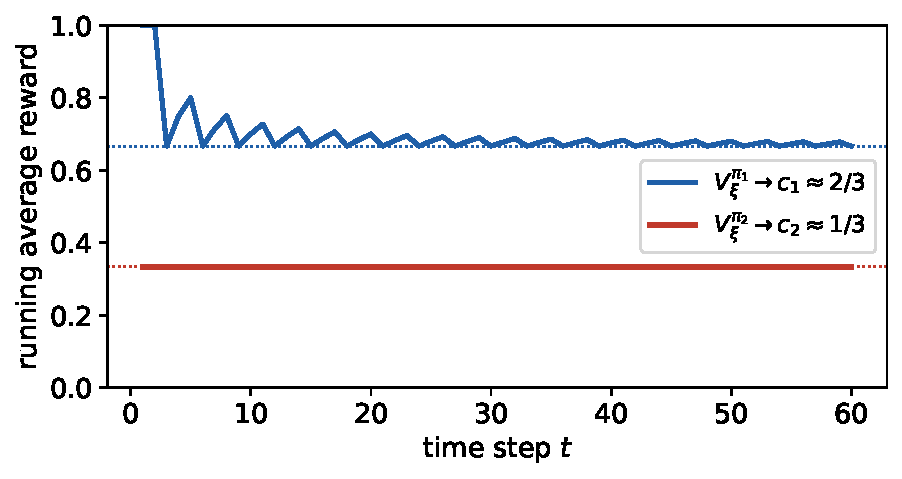
\includegraphics[width=0.62\linewidth]{dogmatic_prior_convergence}
  \end{center}
  Both agents' running average rewards converge to fixed constants:
  $V_\xi^{\pi_1}\to c_1\approx2/3$ (blue) and $V_\xi^{\pi_2}\to c_2\approx1/3$
  (red). By Theorem 8.2.1, dogmatic mixtures $\xi_1',\xi_2'$ then exist
  under which each agent's Bayes-optimal policy \emph{always} sticks to
  $\pi_1$, respectively $\pi_2$ -- since deviating looks catastrophic
  under a dogmatic prior.
\end{frame}

\begin{frame}{Example 10.7.3, Continued: Why This Is Not Nash}
  Since $V_\xi^{\pi_1}\to c_1\approx2/3>0$ and $V_\xi^{\pi_2}\to
  c_2\approx1/3>0$, there is an $\varepsilon>0$ with
  $V_\xi^{\pi_1}>\varepsilon$ and $V_\xi^{\pi_2}>\varepsilon$ for all time
  steps -- both agents are, in this weak sense, doing fine. Yet:

  \vspace{0.3em}
  \textbf{This does not converge to a (approximate) Nash equilibrium.}
  Both agents' values have converged and stabilized (they are locked onto
  fixed constants $c_1\approx2/3$ and $c_2\approx1/3$), yet neither agent
  is actually best-responding: Agent 2 knows (or could learn) that Agent 1
  always plays $(HHT)^\infty$, so Agent 2 could switch to always playing
  the \emph{opposite} of Agent 1's predicted action and get reward $1$
  every single time, instead of $1/3$. Likewise, Agent 1 could switch to
  always playing $H$ (matching Agent 2's constant action) and get reward
  $1$ every time, instead of $2/3$. Because each agent's dogmatic prior
  makes deviating from its own fixed policy look catastrophic (a ``go to
  hell'' event), \emph{neither ever deviates}, and the pair is permanently
  stuck away from any $\varepsilon$-Nash equilibrium.
\end{frame}

\begin{frame}[fragile]{Python: Simulating the Dogmatic-Prior Matching-Pennies Example}
  We simulate $\pi_1=(HHT)^\infty$ against $\pi_2=\pi_H$ (always Heads),
  compute their running-average rewards, and compare against the reward
  each agent \emph{could} get by best-responding instead.
  \begin{lstlisting}[style=pycode]
T = 30
pi1 = [1, 1, 0] * (T // 3)     # H=1,H=1,T=0 repeating
pi2 = [1] * T                  # always Heads (H=1)
r1 = [1 if pi1[t] == pi2[t] else 0 for t in range(T)]  # agent 1: reward if match
r2 = [1 if pi1[t] != pi2[t] else 0 for t in range(T)]  # agent 2: reward if mismatch
avg1, avg2 = sum(r1) / T, sum(r2) / T
print(f"avg reward pi_1 (locked-in) = {avg1:.3f}  (theory: 2/3 = 0.667)")
print(f"avg reward pi_2 (locked-in) = {avg2:.3f}  (theory: 1/3 = 0.333)")
# Best response: agent 2 predicts pi_1 and always plays the OPPOSITE action.
best_r2 = [1 if pi1[t] != (1 - pi1[t]) else 0 for t in range(T)]
print(f"avg reward if agent 2 best-responds = {sum(best_r2)/T:.3f}  (vs 0.333)")
# Best response: agent 1 predicts pi_2 == always H, and matches it.
best_r1 = [1 if 1 == pi2[t] else 0 for t in range(T)]
print(f"avg reward if agent 1 best-responds = {sum(best_r1)/T:.3f}  (vs 0.667)")
# avg reward pi_1 (locked-in) = 0.667  (theory: 2/3 = 0.667)
# avg reward pi_2 (locked-in) = 0.333  (theory: 1/3 = 0.333)
# avg reward if agent 2 best-responds = 1.000  (vs 0.333)
# avg reward if agent 1 best-responds = 1.000  (vs 0.667)
  \end{lstlisting}
  Both agents leave a huge amount of value ($0.667$ and $1$ respectively)
  on the table forever -- exactly the failure Example 10.7.3 describes.
\end{frame}

\begin{frame}{Theorem 10.7.4: Convergence to Equilibrium}
  The following theorem is the main positive convergence result. It
  states that we \emph{do} get convergence to $\varepsilon$-Nash equilibria
  in any reflective-oracle-computable multi-agent environment, provided
  the agents are asymptotically optimal \emph{in mean} (a weaker
  requirement than the dogmatic agents above satisfy).
  \begin{block}{Theorem 10.7.4 (Convergence to equilibrium)}
    Let $\sigma$ be a reflective-oracle-computable multi-agent environment
    and let $\pi_1,\ldots,\pi_n$ be reflective-oracle-computable policies
    that are asymptotically optimal in mean (Definition 8.1.6) in the
    class $\Mc_r^O$. Then for all $\varepsilon>0$ and all
    $i\in\{1,\ldots,n\}$, the $\sigma^{\pi_{1:n}}$-probability that the
    policy $\pi_i$ is an $\varepsilon$-best response converges to $1$ as
    $t\to\infty$.
  \end{block}
  \textbf{Contrast with Theorem 10.7.1.} In contrast to Theorem 10.7.1,
  which yields policies that play a \emph{subgame perfect} equilibrium,
  this is not the case here: the agents typically do not learn to predict
  off-policy, and thus will generally not play $\varepsilon$-best
  responses on the counterfactual histories they never see. This weaker
  form of equilibrium is unavoidable if the agents do not know the
  environment, because it is impossible to learn the parts of it they do
  not interact with.
\end{frame}

\begin{frame}{Corollary 10.7.5: Thompson-Sampling Reflective AIXI}
  Together with Theorem 10.5.4 and the asymptotic optimality of the
  Thompson sampling policy (Theorem 9.2.1), which is reflective-oracle-computable,
  we get the following corollary.
  \begin{block}{Corollary 10.7.5 (Thompson-Sampling reflective AIXI converges to equilibrium)}
    There are limit-computable policies $\pi_1,\ldots,\pi_n$ such that for
    any computable multi-agent environment $\sigma$ and for all
    $\varepsilon>0$ and all $i\in\{1,\ldots,n\}$, the
    $\sigma^{\pi_{1:n}}$-probability that the policy $\pi_i$ is an
    $\varepsilon$-best response converges to $1$ as $t\to\infty$.
    Thompson-Sampling AIXI $\pi_{TS}$ (Algorithm 9.3) with class $\Mc_r^O$
    is such a policy.
  \end{block}
  \textbf{Plain English.} The Thompson-sampling agents $\pi_{TS,i}$ are
  allowed to differ from each other: they can use different discount
  functions, resample at different time steps, and converge at different
  speeds. All of the Thompson-sampling agents eventually ``calm down'' and
  settle on some posterior belief.

  \vspace{0.3em}
  This is a truly remarkable solution to the Grain of Truth problem: the
  \emph{only} assumption on the environment $\sigma$ is computability,
  while reflective AIXI is still merely limit-computable (like single-agent
  AIXI based on $\Mc_{sol}$) -- not practical, but potentially inspiring
  practical versions of this construction. Reflective oracles have already
  seen applications in one-shot games {\footnotesize[FTC15]}.
\end{frame}

%% ══════════════════════════════════════════════════════════════════════════
\section{10.8 Exercises}

\begin{frame}[allowframebreaks]{Exercises}
  \begin{enumerate}
    \item[\textbf{1.}] [C18] Prove Theorem 10.2.4.
    \item[\textbf{2.}] [C28m] Prove Theorem 10.2.7.
    \item[\textbf{3.}] [C20] Prove Theorem 10.2.11.
    \item[\textbf{4.}] [C25] Prove that specific properties (Markov,
      computability, stochasticity, partial observability, optimality
      conditions) carry over in the strategic games to RL conversion (and
      vice versa).
    \item[\textbf{5.}] [C28] Prove that the environment class of repeated
      strategic games admits self-optimizing policies, and hence that
      $\pi^*_\xi$ is self-optimizing over the environment class of
      repeated strategic games.
    \item[\textbf{6.}] [C18] Derive some simple (trivial) environment
      classes where there is a Grain of Truth.
    \item[\textbf{7.}] [C25] Extend the proof of Theorem 10.6.3 to an
      arbitrary finite action space.
  \end{enumerate}
  \vspace{0.4em}
  \textbf{Reading the difficulty codes.} The bracketed code (e.g.\
  [C18], [C28m]) is the book's difficulty rating: roughly, the number
  gives an estimated difficulty out of $50$, ``C'' marks a
  \emph{creative}/research-flavoured exercise, and a trailing letter
  (e.g.\ ``m'') marks additional notes on the exercise's character (such
  as requiring extra mathematical machinery).
\end{frame}

%% ══════════════════════════════════════════════════════════════════════════
\section{10.9 History and References}

\begin{frame}[allowframebreaks]{History and References}
  \textbf{Game theory.} The topic of game theory is well developed in the
  textbook {\footnotesize[OR94]}. It is a theoretical framework
  originating from the work of John von Neumann and Oskar Morgenstern in
  the 1940s, allowing for a theoretical understanding of strategic
  interaction between agents in both competitive and cooperative
  environments {\footnotesize[VNM47]}. Central to game theory is the
  concept of \textbf{Nash Equilibrium}, introduced by John Nash in the
  early 1950s, which describes a state in a strategic game where no
  player can benefit from unilaterally changing strategies while the
  other players keep their strategies unchanged {\footnotesize[NJ50]}.
  This equilibrium is stable, but it may be Pareto dominated by another
  strategy if players can collude to select it.

  \vspace{0.3em}
  This discovery can explain many counter-intuitive results: (1) why
  adding a new road to an existing road network can cause the travel time
  to paradoxically increase for all drivers {\footnotesize[Bra68]}; (2)
  why deliberately limiting the set of available actions via credible
  pre-commitment to a strategy can be advantageous {\footnotesize[Sch80]}.
  It also has applications explaining strategies that evolve naturally in
  the animal kingdom: (3) either passive or aggressive strategies can be
  stable in the animal kingdom {\footnotesize[SP73]}; (4) animals often
  display costly signals, like the peacock's elaborate tail, to help find
  a mate {\footnotesize[Ham64]}; (5) altruistic behaviours can evolve in a
  survival-of-the-fittest framework.

  \framebreak
  \textbf{Mixed strategies and further reading.} Often, a deterministic
  strategy may leave the agent open to being exploited. Mixed strategies
  allow agents to choose a stochastic strategy to avoid exploitative
  responses {\footnotesize[Neu28]}. Besides Nash equilibrium, there are
  other concepts such as altruistic equilibrium and dominant strategy
  equilibrium, and Pareto optimality. A complete classification of
  $2\times2$ symmetric games can be found in {\footnotesize[BWEH22]},
  which covers PD, SH, Chicken, and BoS, but not MP, since the latter is
  not symmetric.

  \vspace{0.3em}
  \textbf{RL and game theory.} The connection between reinforcement
  learning and game theory is presented in {\footnotesize[SLB08]}, which
  includes a survey of MDPs for multiplayer games. Another useful resource
  on this connection is {\footnotesize[Cri17]}, which reviews the
  multi-agent and multi-objective reinforcement learning literatures.
  POTMMCP {\footnotesize[SKH23]} is a theoretically sound multi-agent
  online-learning MCTS-based planning algorithm with good practical
  performance, even for problems requiring a large planning horizon.
  {\footnotesize[MJS19]} considers deterministic games with local Nash
  equilibria (non-zero second derivative of gradient dynamics) and shows
  that gradient descent can get attracted to non-Nash local extrema (or
  saddle points).

  \framebreak
  \textbf{Grain of Truth and reflective oracles.} Finding a grain of truth
  is a famously hard problem {\footnotesize[KL93]}, with many
  impossibility results {\footnotesize[Nac97, FY01, Nac05]}. The
  remarkable solution presented in this chapter is from
  {\footnotesize[LTF16, Lei16b]}, using previous reflective oracle work
  from {\footnotesize[FST15, FTC15]}. Sections 10.3 and 10.5 to 10.7 were
  taken with permission from {\footnotesize[LTF16, Lei16b]}, with some
  minimal modification.
\end{frame}

\end{document}
